\documentclass[12pt]{report}
\usepackage[utf8]{inputenc}
\usepackage{graphicx}
\usepackage[tmargin=2cm, lmargin=4cm, rmargin=2.5cm, bmargin=4cm, paperwidth=8.267in, paperheight=11.692in]{geometry}
\usepackage{amsfonts}
\usepackage{array}
\usepackage{indentfirst}
\graphicspath{ {images/} }
\usepackage{lipsum}
\usepackage{verbatim}
\usepackage{titlepic}
\usepackage{amsmath}
%\usepackage{titlesec}

\begin{document}

\title{Light Field Sampling \vspace{2.5cm}}	%\includegraphics[scale=0.2]{university_edinburgh.jpg}
\author{
\Large Carson Vogt \vspace{1cm} \\ 
}

\date{
	\centering
	PhD Electric Engineering \endgraf\medskip
	Heriot-Watt University \endgraf\medskip
	8 December 2017
}

\maketitle

\listoffigures

\tableofcontents

\chapter{Introduction}

Light field rendering is a fascinating image-based rendering (IBR) technique whose properties have only begun to be explored. With the seminal paper on the topic relatively recently published in 1996 by Levoy and Hanrahan\cite{Levoy96}, research and applications have been rather limited. Early research was focused largely on improving graphics as IBR provides a very immersive and potentially fluid experience for the user, while theoretically relying on very little information of the scene, such as geometry. Of course, as will be discussed, there are times when having extra information like scene geometry can be useful in rendering \cite{Gortler96}. Partly due to the original purpose behind light fields, current research trends have largely been directed towards virtual reality (VR) applications in the entertainment industry \cite{Anderson16, Davis12, Kalantari16}. Apart from attempts at applying light fields to microscopy and depth estimation, few researchers have successfully attempted to apply the light field methodology to other areas \cite{Levoy06b}. There are a number of reasons for the limited research directions and abundance which will be covered here as well as the positive aspects and advantages of light field IBR.

Light fields are a rising method for rendering scenes. With the increasing popularity of VR, light field technology has the potential to revolutionize the way in which viewers interact with subjects of interest.
\begin{figure}[!ht]
	\centering
	\includegraphics[scale=1]{levoy_lf.jpg}
	\caption{ \cite{Levoy96}.}
	\label{fig:levoy_lf}
\end{figure}
McMillan and Bishop describe IBR as the method of creating a "continuous representation" of a scene or subject being discretely sampled \cite{McMillan95}. The sampling that makes up light field IBR is derived from the plenoptic function, a seven-dimensional function that describes the sum of light rays at any point in space \cite{Adelson91}. However, the plenoptic function itself is rarely if ever used in practical applications or research as measuring the full plenoptic function would be impossible. The plenoptic function effectively stopped being used in research in its 7D form with \cite{Adelson91}, but from it the light field was created which allows for descrete parts of the plenoptic function to be measured.

The light field itself was presented by Levoy in 1996 and is a 4D function that is oftened viewed flattened as a 2D array of 2D images. An excellent example of this can be seen in figure \ref{fig:levoy_lf}, and was collected by Levoy and Hanrahan in their early research. After collecting these images, the light field is actually utilized by querying a database of light rays corresponding to the viewpoint of the observer. This requires the camera location to be known very precisely such that when the rays are actually collected and stored, the correct rays can then be utilized when creating the new view. While this is how the methodology is presented in the literature, the story for practical applications is different, and relies instead on a number of assumptions about the light field being collected and blending the resulting images, which will be covered later in the report.

Light fields have a number of intriguing qualities, some of which have yet to be fully exploited. As mentioned before, the most popular quality is the immersive nature of the light field. Taking real images naturally makes it more realistic so long as images are smoothly rendered from the database. another interesting quality comes about due to the large number of images acquired. Occluders within a scene can effectively be erased from the scene, as shown in figure \ref{fig:seethrough_occluder}. While no individual image captured can recreate a complete view of the background, the pieces of the background captured can be combined to recreate it, sometimes entirely removing the occluder from the scene \cite{Vaish06}.
\begin{figure}[!ht]
	\centering
	\begin{minipage}{0.45\textwidth}
		\centering
		\includegraphics[scale=0.55]{seethrough_occluder.png}
		\caption{}
		\label{fig:seethrough_occluder}
	\end{minipage}\hfill
	\begin{minipage}{0.45\textwidth}
		\centering
		\includegraphics[scale=0.55]{seethrough_occluder2.png}
		\caption{}
		\label{fig:seethrough_occluder2}
	\end{minipage}
\end{figure}

There are a number of major limitations associated with light fields currently. To attain the very immersive qualities that makes them appealing, a large number of images must be acquired. If image density is too low, several rendering artifacts can appear, such as hair, pixelation, etc cite{Camahort09}. Papers have been published to decrease the number of required images and will be covered in more detail in the \emph{Literature Review} chapter of the report. Because of the large number of images required, the method for data collection is often bulky or slow \cite{lfArchive}. The light field is further limited by the collectors chosen parametrization, and generally limits the viewer to a planar or spherically based view of the scene \cite{Levoy06a}. 

If one goes back to the original paper regarding the plenoptic function, a critical element is present in it and missing from the current parametrizations: time. Up until recently, light fields have been collected only for static scenes, but advances in light field cameras and processing power have seen small advancements in dynamic light fields \cite{Anderson16, lytro}. Regardless, this still leaves the user with the problem of mobility, where apparatus are fixed and generally must adhere to the strict parametrization around which they were designed. And still, the applications have only been for VR applications.

The project goal is two-fold: one part being to utilize existing research in novel ways to collect and allow for the visualization of dynamic light fields. The second part is to explore novel applications, such as visualizations for the medical field, sports, and other scientific areas such as botany that could benefit from a method of viewing subjects from any point in space \emph{and} time.

\chapter{Literature Review}
The light field is, at its base, a derivation of the plenoptic function (the root \emph{plenus} meaning complete). The plenoptic function, the concept for which was set forward by Adelson and Bergen in 1991, is a method of mathematically describing the elements of vision. The paper takes on the task of defining what can be seen across 3D space, where every point (or "pencil" of rays) contains the information for all of the rays passing through it. This is illustrated well in figure \ref{fig:plenoptic_visual}. 
\begin{figure}[!ht]
	\centering
	\includegraphics[scale=0.75]{plenoptic_image.png}
	\caption{The plenoptic function sampled at two points, showing all pencils of light rays which pass through those points \cite{Adelson91}.}
	\label{fig:plenoptic_visual}
\end{figure}
The concept of all light passing through a point is rooted in the early observations of Leonardo da Vinci, who observes the effect of a hole in a wall, which reveals an image of the scene in front of the wall, upside down on the back wall \cite{Adelson91}. This is the concept behind the pinhole camera, which is a key assumption applied to cameras in much of the work done with light fields. This allows for the use of a ray tracing technique regarding the incoming light rays to a camera. These rays can then be individually stored and queried at a future date for the synthesis of new or old views. The next section discusses the derivation of the 4D light field from the 7D plenoptic function.  

\section{Early Research and Derivation from Plenoptic Function}
Having a basic idea of what constitutes light in space, Adelson and Bergen set forth to mathematically represent this plenoptic function.
The function itself is given as 
\begin{equation}
P=P(\theta,\phi,\lambda,t,V_x, V_y,V_z)
\end{equation}
where $\theta$ and $\phi$ are the viewing angles from a point in space, $\lambda$ is the wavelength of the incoming ray, $t$ is the time parameter at which the ray is observed, and $V_x,V_y,V_z$ define the location in three dimensional space at which the incoming rays are measured \cite{Adelson91}. This defines the incoming rays at every point in 3D space for all time. This would then theoretically allow for the reconstruction of any view, in any space for which the plenoptic function was completely known or measured. However, measuring the plenoptic function comes with its own set of difficulties.

The 7D plenoptic function is a bit impractical to work with, and researchers sought, and continue to seek, to reduce the dimensionality of the function in a number of ways. In \cite{McMillan95} and \cite{Huang14}, the 7D plenoptic function is reduced to five dimensions,
\begin{equation}
p=P(\theta,\phi,V_x,V_y,V_z)
\end{equation}
where $t$ and $\lambda$ are omitted as the time of sampling is considered to be constant (therefore requiring the scene remain static) and the wavelength is constant so long as there are no occluders \cite{Levoy06a}. 

In Levoy and Hanrahan's seminal paper \emph{Light Field Rendering} \cite{Levoy96}, the authors note that in space free of occlusions, the function can be further reduced to a four dimensional function as the ray of light reaching the pixel will not be altered in free space. In this environment, the only requirement is to know the direction of a ray, which is a function of four points shown in the following equation:
\begin{equation}
r=L(u,v,s,t)
\end{equation}
where $r$ is the radiance of an individual ray passing through the planes. This parametrization requires a ray to pass through two known planes, defined as the $s,t$ and $u,v$ planes. This is  still a standard parametrization, used in \cite{Isaksen01}, \cite{Vaish06}, and \cite{Oberlin16}, among others. In one case, a three dimensional parametrization is used as acquisition is completed by using a 1D row of cameras, though obviously this is considerably more limiting than the previous cases, and is considerably less frequently used \cite{Kim13}. Levoy and Hanrahan introduce the 4D parametrization as the "light field" \cite{Levoy96}.

While \cite{Levoy96} introduces the popular two plane parametrization, McMillan and Bishop define a cylindrical parametrization a year earlier. Having encountered difficulties storing a spherical parametrization on a computer, the authors note that with a cylinder, it can effectively be unrolled into a plane, thus making it easy to store and access \cite{McMillan95}. While it may have been easier, it is quickly passed by spherical parametrizations, which offers viewers the ability to also look up. In \emph{Light Fields and Computational Imaging}, Levoy outlines the available parametrizations as of 2006, shown in figure \ref{fig:parameterization_visual}.

With Isaksen et al.'s \emph{Dynamically Reparameterized Light Fields}, a reworking, of the original two plane parametrization was developed, though \cite{Camahort09} argue that it is a separate parametrization altogether. Rather than have two planes in free space, the planes are moved to the internals of the camera, between the lens and the image sensor, guaranteeing the one of the original assumptions, that the space between the subject and the camera be free of occlusions. As well, the authors introduce the concept of not only a mobile focal plane, such as that seen in figure \ref{fig:mobile_focus}, but a focal plane free to change shape and distance according to the user \cite{Isaksen01}. 

\begin{figure}[!ht]
	\centering
	\includegraphics[scale=0.75]{Light-field-parameterizations.png}
	\caption{This image depicts the most common parameterizations at the time ***cite was written. Of the three, the two plane parameterization on the far right persists as the most popular.}
	\label{fig:parameterization_visual}
\end{figure}

\section{Light Field Sampling}
Light field collection has gone relatively unchanged since its inception. Most techniques are a fairly brute force method utilizing a large array of cameras in one form or another. Stanford's New Light Field Archive uses a wall of cameras or a single camera on a gantry \cite{lfArchive}, while companies such as Lytro have developed a spherical bank of cameras \cite{lytro}. An example of this can be seen in figure \ref{fig:camera_array}. This method of capture allows for the light field to be captured quickly and precisely since each camera can capture an image at the same time as every other camera, and the location of each camera is known. However, due to the structure's vast size, moving it to capture interesting scenes is highly impractical, relying on the user to provide huge amounts of power and computing power to an impractical location outside of a lab. While a number of groups have shown interesting use cases for the camera array (some of which will be covered in later sections), it is clearly not a practical method for capturing difficult scenes. While there are some interesting methods for the collection of light fields, they are still quite limited by their parametrizations and the density of the data they must collect \cite{Ihrke16}.

In an effort to decrease the size and complexity of the system, the team at Stanford created a computer controlled, gantry-based, light field collection system \cite{Koller04}. This allowed them to avoid using a complex and relatively immobile capture system in favor of a somewhat more mobile and economical single camera system. Of course, the gantry system is only appropriate for scenes that are static long enough and the light remaining consistent enough for the camera to move through its programmed range of motion. It also removes some of the interesting functions made possible by the array, such as high speed video from multiplexed cameras detailed by Wilburn et al. \cite{Wilburn05}.

Utilizing the growing capabilities of image sensors, Ng shows in his thesis a way by which a light fields can be captured with a single camera. Rather than producing a single image, a microlens array is inserted into the camera. This enables the user to create such effects as refocusing and some minimal movement around the image for a 3D effect after the image has been captured \cite{Ng06, Ng05, Perwass12}. The light field camera trades off spatial resolution in favor angular resolution, although attempts have been made at retaining the spatial resolution \cite{Georgeiv06}.

Another unique data collection method was demonstrated in Davis et al.'s paper, \emph{Unstructured Light Fields} \cite{Davis12}. In it, the authors demonstrate a method for collection utilizing a single camera and a SLAM algorithm known as parallel tracking and mapping, or PTAM \cite{Klein07}. By getting the positional information of the camera via PTAM, the authors instruct a human user on where to move the camera for adequate coverage of a light field. 

Minimizing the amount required to collect(cite review and actual article)
Move on to the more recent papers of Sparse lightfields and learning 
based view synthesis

\cite{Ng06}
\cite{Davis12}
\cite{Oberlin16}


While light field rendering is the most immersive image-based rendering technique, one of the drawbacks of the light field is that the number of images required to create a high resolution and immersive scene can be prohibitively large \cite{Anderson16}. Even Davis et al. admit in \cite{Davis12} that it takes a user several minutes to collect the light field for a subject with their relatively streamlined technique \cite{Davis12}. This leads to the natural question of the amount of sampling required for a complete or usable light field. There is a surprisingly limited number of publications on the subject, which likely has to do with the fact that methods for data collection focus on oversampling and thus it is one of the less-studied areas within the light field field.

\section{Image Interpolation}
As mentioned, one of the drawbacks of light fields is the amount of data required. Without any data interpolation, collection must be very dense, requiring the impractical apparatus mentioned previously. A number of researchers have sought out a solution to the high density issue associated with the hopes of making the acquisition process faster. These methods vary from geometric analysis of light field collection to employing deep learning techniques to interpolate between collected images.

In the paper \emph{Plenoptic Sampling}, Chai et al. set about to describe a minimum sampling rate such that the light field might be completed without any image interpolation. Their method suffers from a rather large flaw, which is that they require the minimum and maximum depths within a scene, and assume that the method for collection is a 2D camera array. Regardless, they manage to present a minimum sampling between cameras in the array given in terms of the resolution of the sampling cameras and renderer (which is assumed to be equal) $\Delta v$ and $\delta v$, and the highest frequency computed from the spectral support $B_v^s$ \cite{Chai00}. 
\begin{equation}
\Delta t_{max} = frac{1}{min \left(B_v^s, 1/(2 \Delta v), 1/2 \delta v)\right) }
\end{equation}

Several other publications make use of geometry when collecting data for a light field. In \emph{The Lumigraph} it is noted that fewer images are required if the collector has some knowledge of the geometry of the scene \cite{Gortler96}. This concept is also made use of in more recent papers, such as \cite{Kim13}. However, such methods are limiting, especially from the perspective of collecting the light field. Ideally, collecting the data should be as hands off as possible. For the purpose of this project the geometric methods are noted, but will not likely be used right away. 

In terms of post processing methods involving image interpolation, there have been a number of relatively new papers which seek to both minimize the number of images taken at the time of collection as well as fluidly complete the light field. In \cite{Shi14}, by analyzing the sparsity in the continuous Fourier domain, show that if light fields are collected to optimize for this, the number of images required to create a light field may be drastically reduced.

In 2016, a paper was published that described a method for employing deep learning to the problem of both collection and then completing the light field. Kalantari et al. trained convolutional neural networks on new view synthesis within light field cameras. Their results suggest that their method, at least on the small scale of a light field camera, produces superior images compared with the previous state of the art. An interesting note by the authors is that, unlike previous methods, use of the CNN means that the new images also carry over the camera artifacts. So while the images themselves might not necessarily be better than previous methods, they do blend in with the real images that were collected by the camera\cite{Kalantari16}. Some very interesting future work would consist of applying this to large scale light fields that might have been collected by robots.

\section{Application of Light Fields}
Graphics and virtual reality are the most obvious and common applications for light fields and have effectively spurred on the field since the middle of the 1990s with the addition of light fields to the IBR repertoire. Few attempts have been made to expand past this, likely due to the fact that those interested in light fields tend to come from graphics backgrounds. However, it is the one of the goals of this project to explore potential applications for light field-based technology.

\begin{figure}[!ht]
	\centering
	\begin{minipage}{0.45\textwidth}
		\centering
		\includegraphics[scale=0.9]{stanford_camera_array.png}
		\caption{The dense camera array used at Stanford to capture a number of light fields.}
		\label{fig:camera_array}
	\end{minipage}\hfill
	\begin{minipage}{0.45\textwidth}
		\centering
		\includegraphics[scale=0.5]{lego_gantry.jpg}
		\caption{Another collection method, the gantry effectively mimics the camera array so long as the scene is not altered between gantry locations.}
		\label{fig:lego_gantry}
	\end{minipage}
\end{figure}
Riding on the work of Ng and the light field camera, Levoy et al. published a paper on light field microscopy \cite{Levoy06b}. Using the light field camera technology, the authors are able to create rather impressive 3D appearing views of the subjects under the lens. By applying the same techniques used in other light field applications, such as synthetic focusing and perspective change, the authors allow for intriguing new ways of viewing biological samples. Of course, as with other light field applications, spatial resolution is limited.

In \cite{Vaish06} Vaish et al. utilize a large camera array to Demonstrate a method by which occlusions can effectively be removed if the light field is sampled densely enough. As well, they do a comparison of different occluders to see at what point an occluder can not be effectively erased from the scene. Examples of this effect can be seen in figures \ref{fig:seethrough_occluder2} and \ref{fig:seethrough_nau}. Applications could be interesting, in the case of monitoring plants, it would be possible to view past certain layers of foliage, or if there is something of interest behind an object that is not in full view in any one image, it can be focused on in the renderer.

Some research has been done in dynamic light fields, but it has been largely untouched. Wilburn et al., utilizing a dense camera array, create a method for creating a high framerate system. However, the large camera array comes with its own set of problems in the form of inconsistent viewing angles causing rendering artefacts, and an inconvenient-to-use system. It is not until 2016 that Google in a paper by Anderson \emph{et al} demonstrated effective light field video, bringing the generally left out time dimension back into the parametrization \cite{Anderson16}. However, it is still fixed to an outward looking spherical parametrization, appropriate for a scene more so than a subject. 

It was Davis et al. who attempted to bring light fields to a consumer level outside of the light field camera concept put forward by Ng. While the use cases are limited, they went as far as developing a mobile application that allowed users to capture their own light field and extract subjects from it as 3D objects \cite{Davis12}. Using a spherical parametrization, inward looking as opposed to the outward looking of the previous paragraph, the authors construct a light field by guiding a user with a graphical user interface that instructs the user on where to hold the camera for data collection.

Working at about the same time as Davis et al., Jachnik et al. create a very similar system. While there are differences in user interface, and algorithmic difference, the concept is quite similar. However, after capturing a light field, the authors attempt to create a crude environment map, and from that the locations of light sources. The results are unique in that for augmented reality applications, shadowing can be implemented on an object that has been placed into a scene, creating a greater sense of realism \cite{Jachnik13}.

\section{Future Collection Methods}
With a few exceptions, the direction of light field capture has largely been constant with researchers relying on the large camera array depicted in figure \ref{fig:camera_array}. While there have been other methods, such as those of Ng, Davis et al., and Jachnik et al., they are either relatively limited in their spatial and angular resolutions, or require significant human interaction to actually create the light field.

Oberlin and Tellex demonstrated the ability to capture a light field with a seven degree of freedom robot arm on a Baxter robot. While there is no doubt that this is a definite move from traditional collection methods, there is a vast amount of research yet to be done in this area with wide ranging applications that could bring light fields to industries outside gaming or virtual reality \cite{Oberlin16}.

The current trend for light field cameras seems to be going in the direction of multi-camera mobile aparatus, as shown in figure \ref{fig:lytro_immerge}
The use cases for these capture methods are similarly limited to the parametrizations used.
\begin{figure}[!ht]
	\centering
	\begin{minipage}{0.45\textwidth}
		\centering
		\includegraphics[scale=0.08]{lytro_immerge.jpg}
		\caption{the lytro immerge, designed to capture an entire scene at once, with an array of cameras built into the structure.}
		\label{fig:lytro_immerge}
	\end{minipage}\hfill
	\begin{minipage}{0.45\textwidth}
		\centering
		\includegraphics[scale=0.12]{jump_vr_video_cameras.jpg}
		\caption{On the right is the camera rig behind the Google Jump VR video system \cite{Anderson16}}
		\label{fig:jump_cameras}
	\end{minipage}
\end{figure}. 

As noted in the introduction, part of the goal of this project is to be able to collect light fields in novel ways. One such potential method is via cameras mounted on one or multiple multirotors, such as the one pictured in figure \ref{fig:ardrone_image}. The amount of research that has gone into multirotor navigation and use as a tool is substantial. A number of those papers were reviewed and could pertain to their use a light field collection devices, covering topics such as trajectory, localization, and data collection. In the first, the previously mentioned PTAM system is integrated into a new navigation system, allowing for fairly accurate localization of the multirotor \cite{Engel12}. Of course, this is key in a mobile image collection application, as pointed out in \cite{Davis12}. Other systems used gauged a scene for optimum light effects and moved appropriately \cite{Srikanth14}, or developed trajectories for multirotors to follow for filming scenes \cite{Roberts16}. Each of these methods use an aircraft to film scenes as precisely as possible, an important quality if such a platform is to be used in the collection of light fields for applications such as inspection of towers or similar structures.

\section{Light Field Photography}
This section goes through, in greater detail, a paper of particular interest written by Ng et al. entitled \emph{Light Field Photography with a Hand-held Plenoptic Camera} \cite{Ng05, Ng06}. In it, the authors outline a method for collecting light fields with a single, modified camera. Using this particular camera allows the authors to avoid the bulky and difficult camera array mentioned previously, while retaining the speed the single traditional camera apparatus loses.

A light field (or plenoptic) camera is virtually the same as a standard camera, with a few very important differences. As with many technologies, image sensors have grown in capability. Sensors of tens of megapixels are not uncommon, and it is this effective over-abundance of sensing power that allows the light field camera to operate. Instead of light going directly to the image sensor to create one large image, light from the lens first encounters a microlens array, which then creates smaller images on the image sensor. Because of this rather major change to the hardware of the camera, software changes must also be made to render images that make use of the modified output from the image sensor. The light field camera can then be thought of as a miniaturized version of the camera array mentioned in previous sections, but without any gaps between cameras, resulting in a more dense light field sampling of the viewed scene.

\begin{figure}[!ht]
	\centering
	\begin{minipage}{0.45\textwidth}
		\centering
		\includegraphics[scale=0.4]{ng_typical.png}
		\caption{the lytro immerge, designed to capture an entire scene at once, with an array of cameras built into the structure.}
		\label{fig:ng_typical}
	\end{minipage}\hfill
	\begin{minipage}{0.45\textwidth}
		\centering
		\includegraphics[scale=0.32]{ng_plenoptic.png}
		\caption{On the right is the camera rig behind the Google Jump VR video system \cite{Anderson16}}
		\label{fig:ng_plenoptic}
	\end{minipage}
\end{figure}.
Ray diagrams are a useful method to better understand the way in which cameras capture information about a scene. They do this by effectively simplifying the path of a ray as it goes from a world plane to the image sensor. Rather than showing a 3D path, the ray space is 2D, showing the intersection of the ray with the lens aperture, $u$, and the image sensor, $x$. Ng uses ray diagrams to show a difference in the way a typical camera captures images, as shown in figure \ref{fig:ng_typical}, and then how a light field camera captures them \ref{fig:ng_plenoptic}. Since each microlens acts like a separate camera across the width of the aperture, considerably more information is gathered about the scene than the traditional camera.

A large section of the paper is dedicated to describing the way in which images are created from the captured light field. The method is described in terms of a synthetic camera, as camera views and focus can vary due to the nature of the light field. The camera uses the parametrization set forward in \cite{Levoy96}, where $L(u,v,s,t)$ describes the ray of light which passes through the lens at $u, v$ and the microlens plane at $s, t$. The authors introduce what they refer to as a "synthetic light field". An excellent visualization is provided by the authors, and is shown in figure \ref{fig:synthetic_image_creation}. With the knowledge of the cameras intrinsic parameters, the irradiance image value is given by the equation 
\begin{equation}
E(s',t')=\frac{1}{D^2} \iint L'(u',v',s',t') A(u',v') cos^4\theta du dv
\end{equation}
with $D$ representing the distance between the synthetic aperture and synthetic film plane, $A$ is a binary aperture function, and $\theta$ is the angle the ray $L'$ makes with the synthetic film plane. Assuming that $\frac{1}{D^2}$ is constant, the term is ignored, as is the $cos^4 \theta$ term, assuming the angles made with the synthetic film plane by the incoming rays are small, then a paraxial approximation can be used. This results in the the following imaging equation:
\begin{equation}
E(s',t')=\iint L'(u',v',s',t')A(u',v')dudv
\end{equation}
In order to put the equation in terms of the light field that has already been acquired, some more geometry is required, and is shown in figure \ref{fig:reference_geometry}
\begin{figure}[!ht]
	\centering
	\includegraphics[scale=0.75]{synthetic_image_creation.png}
	\caption{This image depicts the most common parameterizations at the time ***cite was written. Of the three, the two plane parameterization on the far right persists as the most popular.}
	\label{fig:synthetic_image_creation}
\end{figure}
\begin{figure}[!ht]
	\centering
	\includegraphics[scale=0.75]{reference_geometry.png}
	\caption{This image depicts the most common parameterizations at the time ***cite was written. Of the three, the two plane parameterization on the far right persists as the most popular.}
	\label{fig:reference_geometry}
\end{figure}
From the diagram, two definitions are made for convenience:
\begin{equation}
\gamma=\frac{\alpha + \beta - 1}{\alpha}
\end{equation}
and
\begin{equation}
\delta = \frac{\alpha + \beta - 1}{\beta}
\end{equation}
With these equations, and the knowledge that the ray intersecting both the $u'$ line and $s'$ line also intersects the $u$ line, it can be said that $u = s'+(u'-s')/\delta$. This allows the substitution to be made such that the ray function $L'(u',v',s',t')$ can be rewritten to,
\begin{equation}
L'(u',v',s',t')=L \left( s'+\frac{u'-s'}{\delta}, t' + \frac{v'-t'}{\delta}, u'+\frac{s'-u'}{\gamma}, v'+\frac{v'-t'}{\gamma} \right)
\end{equation}
Substituting again yields what the author refers to as the "Synthetic Photography Equation", and allows for the creation of new images from the light field data:
\begin{equation}
E(s',t')=\iint L \left( s'+\frac{u'-s'}{\delta}, t' + \frac{v'-t'}{\delta}, u'+\frac{s'-u'}{\gamma}, v'+\frac{v'-t'}{\gamma} \right() A(u',v')dudv
\end{equation}
A key feature of the camera is the ability to refocus an image after it has been acquired. To actually accomplish the refocusing, only the synthetic film plane needs to move. In the case where $\beta = 1$, then $\delta = \alpha$, and $\gamma = 1$, and a full aperture is used, such that $A(u',v') = 1$. The synthetic photography equation then becomes 
\begin{equation}
E(s',t') = \iint L \left( u', v', u'+\frac{s'-u'}{\alpha}, v'+ \frac{t'-v'}{\alpha} \right)du'dv'
\end{equation}
showing that only the the $s',t'$ terms need to vary. This method corresponds to one of the renderers discussed in the System Built section.

There are a few drawbacks to the system. As noted by the authors, there is a trade-off by utilizing the sensor image to collect multiple images, and naturally it is that resulting images are of a lower resolution than if a single image had been taken by the image sensor. As well, the spatial and angular data collected is lower than that collected by the standard camera array. As an aside, the authors' focus for the system is largely for entertainment purposes, leaving the technology lying in wait for some novel application that has yet to be realized.

\chapter{Progress to Date}
From the start of the project, practical work has been important alongside learning the theory and past work done via the literature review and applying some techniques from the literature. A considerable amount of work has been done so far in terms of learning signal processing and optics, constructing light field viewers, and creating a code base out of current state of the art techniques and technologies. This sections covers several of the blocks that make up the base of current and future research. It covers some of the hurdles encountered in deducing what platforms to use, such as quantifying the accuracy of the systems involved and comparing them. As well, light fields were collected throughout the process using various methods during the platform exploration. Finally, several different light field viewers, or renderers, were created using different techniques and parametrizations covered earlier in the paper, but will be lightly reviewed again in the coming section.

\section{Comparison of Platforms}
As discussed in the previous section, methods for collecting light fields are varied. Several of the existing methods are too expensive or time consuming to attempt, such as building a large camera array, or assembling a mobile gantry equipped with a camera. Do to the unique access to several different robot platforms, a couple methods have been thoroughly explored and are discussed here. Much of the time was spent exploring acquisition via humanoid robot, such as the Baxter and PR2 robots \cite{baxter, PR2}. Future work will certainly include a UR10 or UR3 robot \cite{UR10}, however time is still being spent writing to software to appropriately control these arms. Each robot has used a readily available USB camera. For all of the rendering methods and future work, camera location precision is key in querying a ray database for appropriate rays for new view creation. However, I show in this section that accuracy is also important or more important as going to a particular location allows more exact sampling of the light field. Therefore, in an attempt to acquire light fields with precise and accurate position values, a comparison was done between what was at the at the time the most available and standard SLAM software, and the Baxter and PR2 humanoid robots. 

\begin{figure}[!ht]
	\centering
	\includegraphics[scale=0.55]{bax_image.jpg}
	\caption{An image of the baxter robot used to acquire some of the first data sets.}
	\label{fig:baxter_image}
\end{figure}

\subsection{Baxter and PTAM}
The first platform tested was the Baxter, equipped with two 7 DOF arms as shown in figure \ref{fig:baxter_image}. Initially, one of the built in cameras was used, similar to using a USB camera. The experiment setup was as follows: a laser was grasped by the robot and directed at a black frame of known dimensions on a white background. Several different patterns were attempted for use, but when vision processing was being done, the black frame target was clearly superior. The arm was programmed to move in a grid pattern, stopping periodically at predetermined points/intervals so that the embedded camera could take a picture of the scene with the laser dot corresponding to the position of the arm. The pictures were then analyzed for accuracy against the predetermined points that the laser should have aligned with. The results of these tests can be seen in figures \ref{fig:bax_ptam_variance} and \ref{fig:bax_ptam_std_dev}. One of the key assumptions is that the camera was far enough from the frame and the movements were small enough that relative distances remained consistent.

\begin{figure}[!ht]
	\centering
	\includegraphics[scale=0.55]{bax_and_ptam_std_dev.png}
	\caption{In this figure, the variance for the different methods, ie Baxter and PTAM are shown. Baxter is the blue column, and PTAM is the black. Clearly, in terms of localization, Baxter is superior to PTAM.}
	\label{fig:bax_ptam_std_dev}
\end{figure}

\begin{figure}[!ht]
	\centering
	\includegraphics[scale=0.55]{experiment_image.png}
	\caption{This figure shows the most complex part of the experiment, where PTAM has been initialized, and Baxter is running through its image collection program.}
	\label{fig:experiment_image}
\end{figure}

In addition to using Baxter's internal position estimation, the PTAM library was used to localize the camera. An example of the experiment apparatus with PTAM running can be seen in figure \ref{fig:experiment_image}. This technique has been used in a number of papers and is seen as a reasonable method for collecting position data. However, references regarding the precision of the SLAM system are difficult to come by. Therefore, it felt appropriate to do a comparison between PTAM and the Baxter's knowledge of its own position. An experiment was therefore set to get adequate data from PTAM for comparison. For the experiment, similar apparatus was used as in the Baxter experiment, with the addition of a large number of features and points for PTAM to recognize. The PTAM positions were then compared against the ground truth laser and frame measurements. 

The results can be seen in figure \ref{fig:bax_ptam_std_dev}. Interestingly, the experiments were run over three Baxter speeds in an attempt to see whether or not precision varied with speed as well as by platform. The figures of the resulting data indicate that Baxter (in blue) is superior in terms of both accuracy and precision, and PTAM (shown in black) being the worst. PTAM also varied highly with the speed at which Baxter was moving. This could be an effect of the camera, but the results do not match intuition as PTAM consistently, over 20 runs of the experiment, performed especially poorly at the middle speed. After the experiments were performed, a new SLAM method was introduced, after eight years of PTAM being the standard, called ORB-SLAM2 \cite{Mur-Artal15}.

\subsection{Accuracy, ORB-SLAM2 and the PR2}
In the second round of testing, greater emphasis was put on the accuracy of the system. Specifically, I define accuracy as the mean offset of the robot from the point it was instructed to go to. The grid defined by the program is made up of three rows of equally distributed points, with the first row being offset to the right by one point. This can clearly be seen in figure \ref{fig:bax_and_lase}. Keeping in mind that the points should be horizontal, it is clear that Baxter is not capable of consistently reproducing the pattern it is programmed to accomplish. This is likely due to the fact that the Baxter is a "safe" robot. That is, its arms are suspended on springs that allow for it to bounce off of objects, rather than forcibly collide with them or attempt to go through them.

\begin{figure}[!ht]
	\centering
	\includegraphics[scale=0.35]{baxter_and_laser.png}
	\caption{Shows the location of the laser (on the left) and where Baxter estimates its position to be (right).}
	\label{fig:bax_and_lase}
\end{figure}

\begin{figure}[!ht]
	\centering
	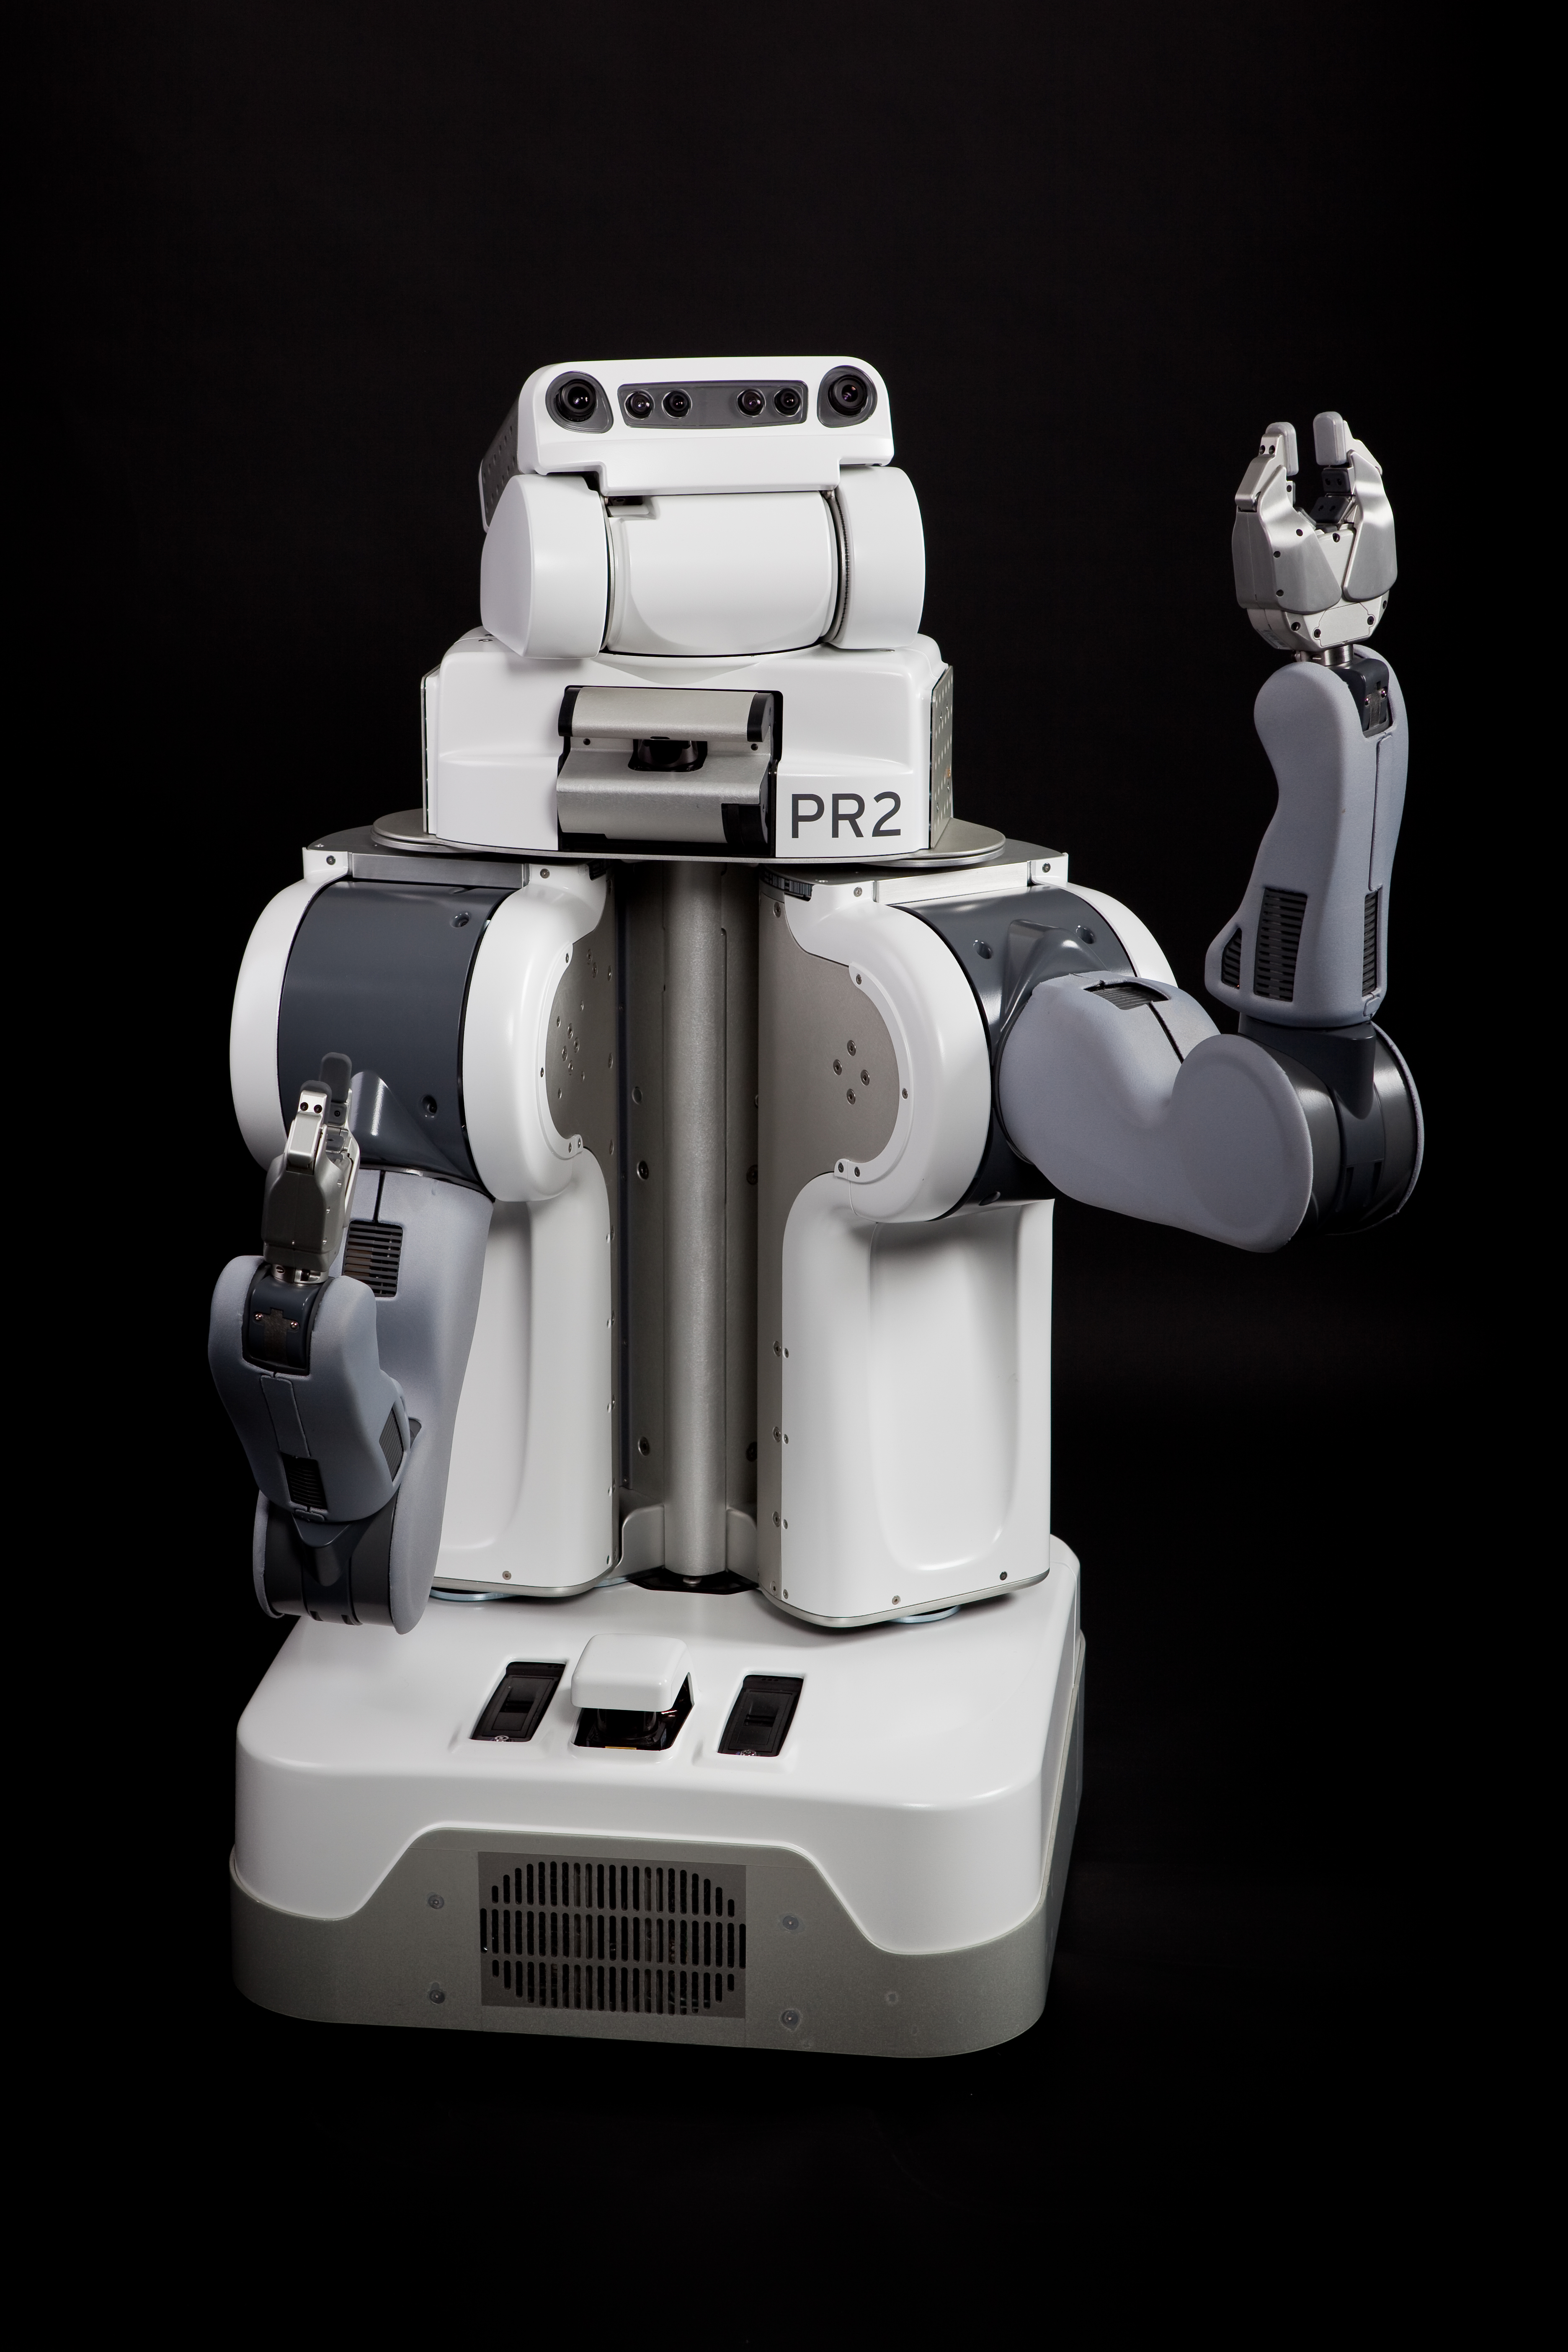
\includegraphics[scale=0.08]{pr2_image.jpg}
	\caption{The second robot platform tested is the PR2. My hypothesis going into testing with it is that it will be considerably more accurate and precise than the Baxter.}
	\label{fig:pr2_image}
\end{figure}

In terms of minimally sampling the light field, Baxter does not seem like an appropriate platform going forward. This then leads into the next question, as to which platform is best. With access to a PR2 robot, shown in figure \ref{fig:pr2_image}, it was then tested. The results from an accuracy test are obvious, as shown in figure \ref{fig:PR2_and_lase}. 

\begin{figure}[!ht]
	\centering
	\includegraphics[scale=0.45]{pr2_and_laser.png}
	\caption{Shows the location of the laser (on the left) and where PR2 estimates its position to be (right).}
	\label{fig:PR2_and_lase}
\end{figure}

\begin{figure}[!ht]
	\centering
	\includegraphics[scale=0.45]{os2_and_laser.png}
	\caption{Shows the location of the laser (on the left) and where ORB-SLAM2 estimates its position to be (right).}
	\label{fig:OS2_and_lase}
\end{figure}

Different SLAM techniques have come to be of particular interest after the rather poor performance of PTAM relative to the Baxter robot discussed in the previous section. An adequate SLAM algorithm will likely be key in determining the method by which data is collected for light fields. As mentioned in the previous section, PTAM was tested alongside Baxter, but according to the acquired data and analysis, it is inferior to Baxter's onboard position estimator. After the first year review, ORB-SLAM2 was tested. ORB-SLAM2 has been touted as a significant step forward from PTAM. My tests prove that while considerably easier to use, for the application of localization for light field images, it is clearly inferior still to both Baxter and PR2. The results of a test can be seen in figure \ref{fig:OS2_and_lase}. While the camera was being moved by the Baxter, ORB-SLAM2 was providing the pose estimates. It is clear from simply looking at the graph that on large scales in might be an adequate system, but for the small, precise movements required for small light field subjects, it is inferior.

\begin{figure}[!ht]
	\centering
	\includegraphics[scale=0.45]{bax_pr2_compare.png}
	\caption{An accuracy comparison between the Baxter and PR2.}
	\label{fig:bax_and_pr2_compare}
\end{figure}

The next question then asks which is more precise, the PR2 or Baxter. A test was done for this as well, the results for which can be seen in figure \ref{fig:bax_and_pr2_compare}. The results were actually very surprising as it turns out that the precision between the two robots is not only comparable, but it is almost equal. This means that both the PR2 and Baxter have nearly equivalent localization estimation error magnitudes, but in terms of accuracy regarding going to a particular location, the PR2 is superior. This will be especially important going forward as light fields may need to be accurately and precisely sampled to acquire the minimal number of images for reconstruction.

\section{Collected Light Fields}
With the results of the platform comparison completed for the time being, a number of light fields were collected to be used with the rendering systems built. The systems themselves are covered in more detail in the next section. 

An example of the type of light field captured can be seen in figure \ref{fig:nau_collected_images}. The result is an array of 2D images of a nau robot. The text in the upper left hand corner of each picture notes the position of the camera according to Baxter. It is used purely for visualization purposes that will become clearer in the next section. The location stamps are based on Baxter's internal position estimation, which was found to be superior to other tested methods in the first section of this chapter.

\begin{figure}[!ht]
	\centering
	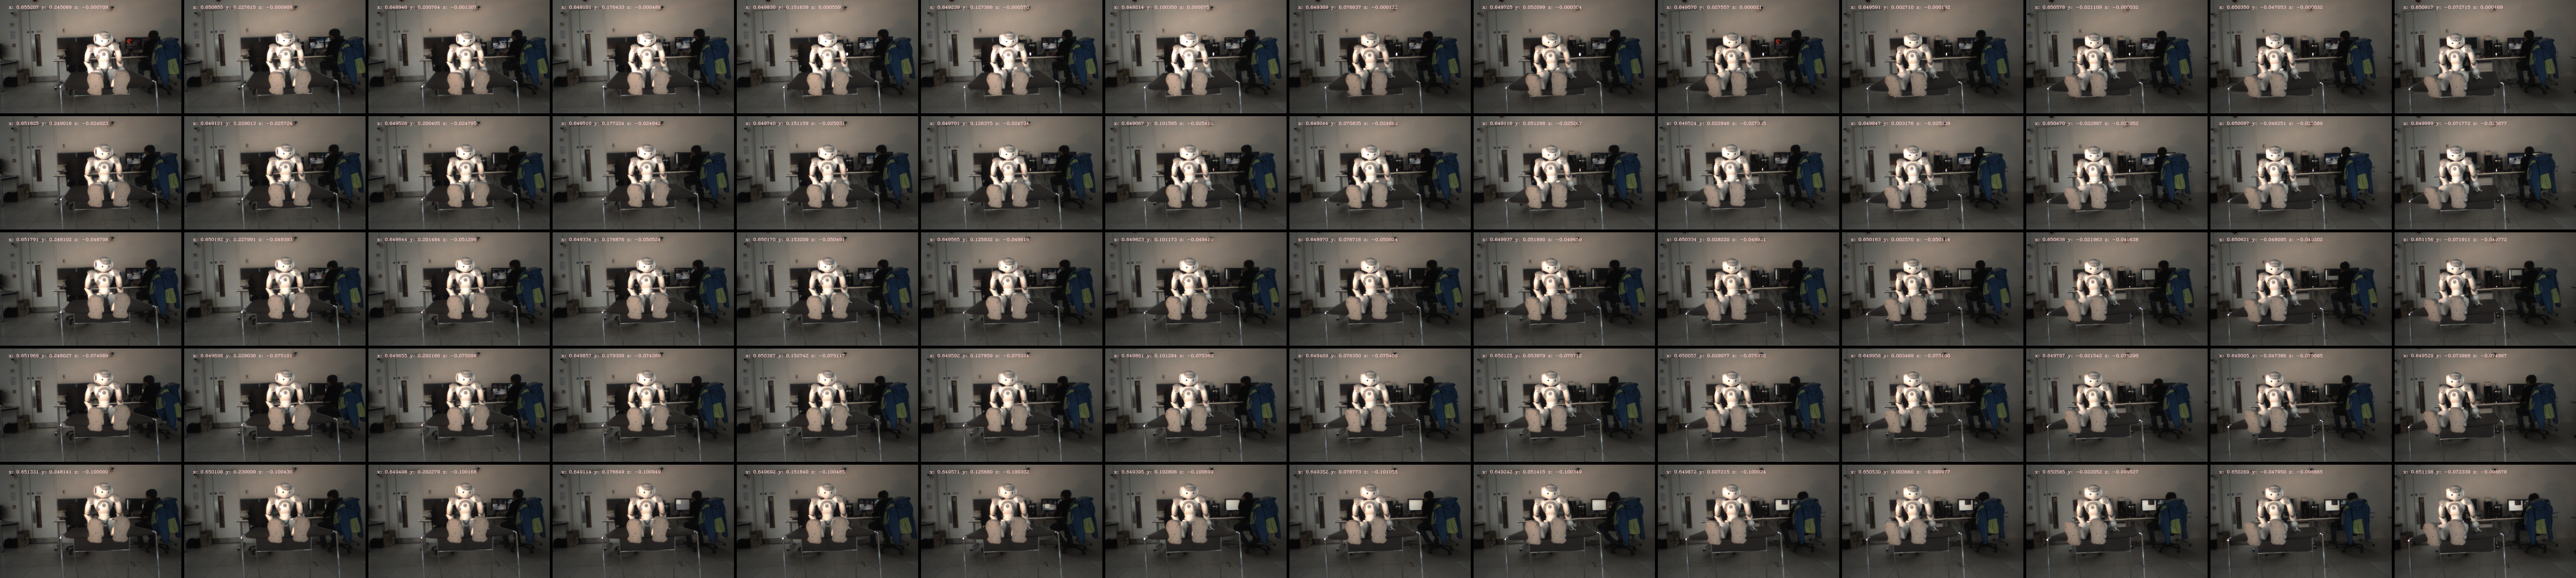
\includegraphics[scale=0.045]{mosaic.jpg}
	\caption{This mosaic is a compilation of all the images taken during one light field acquisition session with the baxter robot.}
	\label{fig:nau_collected_images}
\end{figure}
There were a number of other light fields collected in a similar manner, each of which had varied scene parameters. While the light field in figure \ref{fig:nau_collected_images} is superior to the other collected light fields, it was a beneficial experiment in understanding what a good light field might look like. In other collected light fields, a plastic skull was used in place of the nau. Lighting and distance were also varied, resulting in approximately ten light fields being collected for experimentation. 

\begin{figure}[!ht]
	\centering
	\includegraphics[scale=0.2]{raytrix_raw.png}
	\caption{A depiction of the second renderer based on \cite{Isaksen01} and showing the plane of focus $F$ and the rays coming from it that would be considered in focus.}
	\label{fig:raytrix_raw}
\end{figure}
A Raytrix r5 camera was acquired and has been used to capture light fields as well. A raw example of this can be seen in figure \ref{fig:raytrix_raw}. In it, the microlenses can clearly be seen, resulting in an almost honeycomb like appearance in the resulting image. The image, being raw, has not gone through any of the software processing similar to that described in the \emph{Light Field Photography} section of the report. Therefore, the image is purely the output from the high resolution image sensor \cite{Perwass12}. Unfortunately, it has proven to be quite difficult to extract classic "stuv" images from the resulting raw Raytrix image. Several attempts were made to identify each of the lenslets, and pull pixels from each of those to recreate the light slab.

\section{System Built}
The following section describes light field renderers that have been successfully constructed to date. Three different systems have been built and iterated upon, and utilize three distinct methods for storing rays and querying a database for the appropriate ray parameters. The first system built takes its form from the seminal paper by Levoy and Hanrahan \cite{Levoy96}, the second is based on the work by Isaksen et al. \cite{Isaksen01}, and the third is a combination of the first system and the renderer created by the New Stanford Light Field Archive \cite{lfArchive}.
\begin{figure}[!ht]
	\centering
	\includegraphics[scale=0.7]{mobile_focus.png}
	\caption{A depiction of the second renderer based on \cite{Isaksen01} and showing the plane of focus $F$ and the rays coming from it that would be considered in focus.}
	\label{fig:mobile_focus}
\end{figure}

The first renderer utilizes the common, and original two-plane parametrization set forward in \cite{Levoy96}. As with all available parameterizations, a pinhole model is assumed for the camera being used. A number of known values are required for this particular parametrization to work, such as distance of the subject from the camera. With this knowledge, the $ST$ and $UV$ planes may be appropriately placed such that light rays from the subject pass through both before entering the camera. Aside from the distance to the subject, the internal physical camera parameters must be known, such as the size of the image sensor, the camera flange focal length, the position of the camera in a global reference frame, and the number of pixels on the image sensor. Knowing these parameters allows for the storage of two points which are defined by the two planes $P=(S,T), Q=(U,V)$, and together give the direction of the ray along with its recorded intensity value. The new ray database can then be queried at any time for a new camera position. With the new position, a k-Nearest Neighbors (KNN) algorithm is used to compare ray directions with stored directions and an average is taken of intensity values for the nearest rays to create a new image.
\begin{figure}[!ht]
	\centering
	\includegraphics[scale=0.4]{nau_lf.png}
	\caption{A screenshot of the light field interface in action, with the subaperture views shown in blue, the aperture shown as the red circle, and the resulting image shown in the larger window.}
	\label{fig:light_field_system}
\end{figure}
\begin{figure}[!ht]
	\centering
	\begin{minipage}{0.45\textwidth}
		\centering
		\includegraphics[scale=0.30]{nau_occluding.png}
		\caption{The dense camera array used at Stanford to capture a number of light fields.}
		\label{fig:nau_occluding}
	\end{minipage}\hfill
	\begin{minipage}{0.45\textwidth}
		\centering
		\includegraphics[scale=0.30]{seethrough_nau.png}
		\caption{Another collection method, the gantry effectively mimics the camera array so long}
		\label{fig:seethrough_nau}
	\end{minipage}
\end{figure}

The second renderer built is based on \cite{Isaksen01}. It is similar to the previous method but moves the planes to the internals of the camera where there are still no occlusions. Regardless of the plane locations, rays from the scene are still calculated and stored the same way, but there is the addition of a mobile "focus plane". This focus plane allows for focus at different points in the scene via finding the rays coming from the object at the plane position as illustrated in figure \ref{fig:mobile_focus}.

A third renderer was built based on \cite{Levoy96} and the online viewer found on the New Stanford Light Field Archive website \cite{lfArchive}. After downloading the ActionScript/MXMLsource code and reverse engineering tt, it was rewritten in C++ and OpenCV. It is pictured in figure \ref{fig:light_field_system}. It is a much simplified version of the first renderer that was programmed, but is considerably faster in its run time. In this case, the images are required to be taken specifically from a single plane as any deviation would lead to ghosting. This is caused by the fact that the current rendering technique that this is based on 

\begin{figure}[!ht]
	\centering
	\includegraphics[scale=0.50]{new_system.png}
	\caption{Image of a Nau posing for the spherical parameterization collection. Individual images are shown in the sub-aperture view and are denoted by the blue squares.}
	\label{fig:spherical_nau}
\end{figure}

Variations on a fourth system were also built. The first results of this most recent system can be seen in figure \ref{fig:spherical_nau}. This follows the same "point-and-collect" method as the previous renderers, however the parameterization is different. This one uses a spherical parameterization, where Baxter has moved around the subject as if the camera were on a sphere. For rendering purposes, it is assumed that each image is taken at a constant depth. This allows for a 2D sub-aperture view with the x-axis being the spherical theta values, and the y-axis being the spherical phi values. Using a graphics geometry library, these images are then triangulated using a Delaunay triangulation, and novel images are created using a barycentric interpolation technique.

\begin{figure}[!ht]
	\centering
	\includegraphics[scale=0.45]{continuous_collect.png}
	\caption{The most recent version of the rendering algorithm where the robot moves continuously and captures very dense data. Shown in the sub-aperture view is approximately half of the actual captured views, with the other half having been taken out in a uniformly random pattern for testing.}
	\label{fig:const_move}
\end{figure}

The most recent version follows the same rendering techniques as the previous version, but is different in two major ways. The first, is that it no longer relies on the "point-and-collect" method, but instead retrieves a constant stream (ie video) of the subject as it follows a trajectory made up of pre-determined waypoints. This allows for extremely dense collection of images, as shown in figure \ref{fig:const_move}. For research going forward, this is very important as it allows for the removal of data, and testing of rendering methods on different densities of images. Another way in which this method differs is in the number of parameterizations used. Models of the three most common, two-plane, spherical, and cylindrical, have been programmed in for data collection. This, however, brings up the next issue: which of the parameterizations is best for a detailed view of a subject? This leads into the final chapter.

\chapter{Research Going Forward}
\section{Analysis of Ray Space}
The first step looks to analyze the paper by Davis et al \cite{Davis12}. In the paper, the authors create a light field collection system that is "unstructured", or one in which the camera positions are not fixed in a grid. This is accomplished by using PTAM alongside a graphical user interface to instruct a human on where to move the hand held camera. The authors are able to use PTAM as the renderer they use does not require the precise position measurements, similar to that of the third renderer discussed in the \emph{Systems Built} section. As well, using video to capture large amounts of data means that errors in rendering are more easily covered. Therefore, it can be deduced that a potential substitute for poor position data is oversampling of the light field. In the future, their technique may prove to have more impact should SLAM techniques improve. However, it is one of the few papers that utilize a spherically parameterized light field, which begs the question, why? A brief analysis of the parameterizations was undertaken, specifically between the spherical and two plane parameterizations. While they each have their applications, the two plane method was developed more as a response to the method in which light fields were captured, ie via a dense camera array. To analyze an individual subject, it was hypothesized that a spherical parameterization would be superior. In this case, superior is defined as the number of rays captured emanating from the subject. To start, a formula was derived for the 2D case, with a simplified subject being represented by a sphere. An earlier practical example of this can be seen in figure \ref{fig:ray_dense_1}.

For the spherical case $C_x =$ is defined as the x coordinate of the subject center, $C_y =$ is the y coordinate, $r_{sub} =$ is the subject radius. $C_{sx} =$ is the x coordinate of the center of the camera circle, and $C_{sy} =$ is the y coordinate, with $r_{sph} =$ representing the camera circle radius.
$$\int_{0}^{2\pi} \phi(\theta) d\theta$$
$$\phi(\theta)=2*sin^{-1}(\frac{r_{sub}}{distance}$$
$$distance=\sqrt{(C_x-x)^2+(C_y-y)^2}$$
$$x = r_{sph}*cos(\theta) + C_{sx}$$
$$y=r_{sph}*sin(\theta)+C_{sy}$$
Put together, this yields the following integral over the sphere yielding the relative area of rays for this particular parameterization.
$$2*\int_{0}^{2\pi} sin^{-1}(\frac{r_{sub}}{Acos(\theta)+Bsin(\theta)+C}) d\theta$$
where $A, B, C$ are constants

For the two plane parameterization, the planes are defined as lines and the subject again is simplified to a circle. However, to make the two equations comparable, the u coordinate for the parameterization was substituted for a phi value. In this case, $t$ is kept constant.

$$\int_{-\infty}^{\infty} \phi(s) ds$$
$$\phi(s)=2sin^{-1}(\frac{r_{sub}}{distance})$$
$$distance=\sqrt{(C_x-t)^2+(C_y-s)^2}$$
$$distance=s^2-2C_ys+Const$$

And the resulting equation is an integral from negative infinity to positive infinity, producing the area of the rays in terms of phi.

$$2*\int_{-\infty}^{\infty} sin^{-1}(\frac{r_{sub}}{s^2-2C_ys+Const}) ds$$

%Looking at ray density
\begin{figure}[!ht]
	\centering
	\includegraphics[scale=0.45]{init.png}
	\caption{An initial view of the rays intersecting a subject. the angle the ray takes is defined by phi, as is the angle between a line from the camera position to the center of the subject.}
	\label{fig:ray_dense_1}
\end{figure}

To finish, the areas taken up by the rays were compared in the form of a ratio with the area covered for the spherical representation in the numerator, and the planar representation in the denominator. This can be seen in figure \ref{fig:ray_dense_2}.

\begin{figure}[!ht]
	\centering
	\includegraphics[scale=0.40]{final_2d.png}
	\caption{In this figure, the left hand side shows a ratio of areas covered by the two parameterizations, with the two plane area in the numerator. It is clear from this that the smaller the distance between the cameras and the subject, the more appropriate it is to use a spherical parameterization.}
	\label{fig:ray_dense_2}
\end{figure}

In the future, more work will be done to analyze the three dimensional case, with the addition of a cylindrical parameterization. I believe that this knowledge is key in understanding which parameterization is best fitted for what a user might be trying to do with the subject, such as 3D reconstruction, textural analysis, sparse sampling, or detailed visual reconstruction.

\section{Creation of a Uncertainty-Based Renderer}
With the tentative knowledge that the spherical parameterization is superior for attaining detailed information about the subject, a dense light field was captured of a subject to create a baseline data set to test rendering methods with. A specific example of that can be seen in figure \ref{fig:images_compared}. In the figure, the top image is an original image from the light field. To test the rendering method, a percentage of the images were removed from the light field, and novel images were rendered in their place based on the previously described barycentric interpolation method. These two images are then compared by calculating the L2 normal.
%Comparison of images
\begin{figure}[!ht]
	\centering
	\includegraphics[scale=0.50]{compared_images.png}
	\caption{This is an example of the typical error comparison. The image on top is the original image that is one of the ten percent of images removed from the light field. It is compared with the novel image created in its original location.}
	\label{fig:images_compared}
\end{figure}

By performing this test on various percentages of removed images, an idea for how successful the renderer is at various percentages is acquired. This is illustrated in figure \ref{fig:error_values}. It can be clearly seen in the figure that the error increases exponentially with the percentage of images removed from the light field, while the standard deviation only increases linearly.

\begin{figure}[!ht]
	\centering
	\includegraphics[scale=0.50]{error_values.png}
	\caption{The top image shows the L2 error for each percentage of images removed from the light field. The bottom image shows the increase in the standard deviation as a function of the percentage of images removed. Interestingly, the error mean increases exponentially, while the error standard deviation seems to increase linearly.}
	\label{fig:error_values}
\end{figure}

\begin{figure}[!ht]
	\centering
	\includegraphics[scale=0.50]{l2_error.png}
	\caption{This shows the shape of the error curve for all of the images at a particular percentage (in this case, ten percent of the images have been removed from the light field). It most closely matches a log normal curve.}
	\label{fig:l2_error}
\end{figure}

From the previous work, we can see that error values are quite clearly displayed for the robot. The next step is to ask if the rendering error can be decreased by propagating the uncertainty from the robot through to the barycentric coordinates. As a side note, it might seem like there are other techniques that have been applied to light fields that might take this into account. In truth, most renderers apart from the unstructured light fields renderer previously mentioned, rely on a structured light field. That is, they required that the images are uniformly spaced, such as the light field obtained by a camera array, or that of a light field camera. Some work has so far been done to characterize the error of the PR2 while continuously collecting images.

%y directional values
\begin{figure}[!ht]
	\centering
	\includegraphics[scale=0.35]{pr2_z_error.png}
	\caption{In this figure, the robots z directional error is shown from horizontal (y direction) movements.}
	\label{fig:pr2_z}
\end{figure}

\begin{figure}[!ht]
	\centering
	\includegraphics[scale=0.35]{pr2_y_error.png}
	\caption{The top images shows the y directional error when the robot is moving left. The bottom images shows the y directional error when the robot is moving right.}
	\label{fig:pr2_y}
\end{figure}

Based on these errors, the next step is to modify the existing barycentric interpolation to account for uncertainty in the measurements. While this has yet to be done, the problem is defined. As well, the barycentric coordinates can be defined by a linear system:
$$\begin{vmatrix}
x_1 &x_2 &x_3 \\ 
y_1 &y_2 &y_3 \\
1 &1 &1
\end{vmatrix}
\begin{vmatrix}
\lambda_1 \\
\lambda_2 \\
\lambda_3
\end{vmatrix}
=
\begin{vmatrix}
x \\
y \\
1
\end{vmatrix}
$$
which can be simplified to 
$$A\lambda=p$$
Most of the literature allows for propagation of uncertainty in the lambda term, yielding
$$
A^{-1}\Sigma \lambda A=\Sigma p
$$
However, there is actually uncertainty in the $A$ matrix as well as the $\lambda$ vector. 

\section{Next Steps}
By modelling the error distribution, there are two potential contributions that can be made in the relatively short term. First, there is a model of the error as the robot moves, potentially allowing for a more accurate knowledge of the location of the camera. This would likely lead to a superior rendering method. As well, because the error is directional, as shown in figures \ref{fig:pr2_y} and \ref{fig:pr2_z}, this allows for the possible definition of paths that the robot might take to minimize the error as the robot moves to collect images. While some of the modelling has already been done, a more robust method has been created to log the locations of the arm. This means that a three dimensional, multi-directional model of the uncertainty of the arm can be created with sufficient data points. The immediate next steps are to analyze the data from the 3D tests (which has already been collected as of the writing of this report) and create an error distribution that is a function of the robot arm direction. The second is to propagate the error through the linear system defining the barycentric coordinates. The final step then is to apply the uncertainty model to the previously collected light field and compare the error values to those in figure \ref{fig:error_values}.

\begin{thebibliography}{10}%Any two digit number for more than nine references

\bibitem{Adelson91}
	Adelson, Edward H. \emph{The Plenoptic Function and Elements of Early Vision} (1991). Computational Models of Visual Processing, pp. 3-20.

\bibitem{Anderson16}
	Anderson, R., Gallup, D., Barron, J. T., Kontkanen, J., Snavely,  N., Hernandez, C., Agarwal, S., and Seitz, S. M., \emph{Jump: Virtual Reality Video} (2016). SA '16 Technical Papers.

\bibitem{Bolles87}
	Bolles, R. C., Baker, H. H., and Marimont, D. H., \emph{Epipolar-Plane Image Analysis: An Approach to Determining Structure from Motion} (1987). International Journal of Computer Vision, no. 1, pp. 7-55. 

\bibitem{Camahort09}
	Camahort, E., Abad, F. and Fussell, D., \emph{A line-space analysis of light-field representations} (2009). Graphical Models. no. 71. pp. 168-183.

\bibitem{Chai00}
	Chai, J., Tong, X., Chan, S., and Shum, H., \emph{Plenoptic Sampling} (2000). SIGGRAPH '00, pp. 307-318.

\bibitem{Davis12}
	Davis, A., Levoy, M., and Durand, F., \emph{Unstructured Light Fields} (2012). Eurographics 2012, no. 31.

\bibitem{Engel12}
	Engel, J., Sturm, J., and Cremers, D., \emph{Accurate Figure Flying with a Quadrocopter Using Onboard Visual and Inertial Sensing} (2012). IEEE/RJS International Conference on Intelligent Robot Systems, no. 320.

\bibitem{Georgeiv06}
	Georgeiv, T., Zheng, K. C., Curless, B., Salesin, D., Nayar, S., and Intwala, C., \emph{Spatio-Angular Resolution Tradeoff in Integral Photography} (2006). Eurographics Symposium on Rendering

\bibitem{Gortler96}
	Gortler, S. J., Grzeszczuk, R., Szeliski, R., and Cohen, M. F., \emph{The Lumigraph} (1996). SIGGRAPH '96, pp. 43-54.
	
\bibitem{Huang14}
	Huang, Z. and Sanderson, A., \emph{Light field modelling and interpolation using Kriging techniques}	(2014). Society of Light and Lighting, no. 46, pp. 219-237.
	
\bibitem{Ihrke16}
	Ihrke, I., Restrepo, J. and Mignard-Debise, L., \emph{Principles of Light Field Imaging} (2016). IEEE Signal Processing Magazine.
	
\bibitem{Isaksen01}
	Isaksen, A., McMillan, L., and Gortler, S. J., \emph{Dynamically Reparameterized Light Fields} (2000). SIGGRAPH '00, pp. 297-306.

\bibitem{Jachnik13}
	Jachnik, J., Newcombe, R. A., Davison, A. J., \emph{Real-Time Surface Light-field Capture for Augmentation of Planar Specular Surfaces} (2013). ISMAR.
	
\bibitem{Joubert15}
	Joubert, N., Roberts, M., Truong, A., Berthouzoz, F. and Hanrahan, P., \emph{An Interactive Tool for Designing Quadrotor Camera Shots} ACM Transactions on Graphics, no. 34. 

\bibitem{Kalantari16}
	Kalantari, N. K., Wang, T. and Ramamoorthi, R., \emph{Learning-Based View Synthesis for Light Field Cameras} (2016). SIGGRAPH Asia '16.

\bibitem{Katayama95}
	Katayama, A., Tanaka, K., Oshino, T. and Tamura, H., \emph{A Viewpoint Dependent Stereoscopic Display Using Interpolation of Multi-Viewpoint Images} (1995). SPIE. no. 2409.
	
\bibitem{Kim13}
	Kim, C., Zimmer, H., Pritch, Y., Sorkine-Hornung, A. and Gross, M., \emph{Scene Reconstruction from High Spatio-Angular Resolution Light Fields} (2013). ACM Trans. Graph.	
	
\bibitem{Klein07}
	Klein, G. and Murray, D., \emph{Parallel Tracking and Mapping for Small AR Workspaces} (2007). ISMAR 2007. 	

\bibitem{Koller04}
	Koller, D., Turitzin, M., Levoy, M., Croccia, G., Cignoni, P. and Scopigno, R., \emph{Protected Interactive 3D Graphics via Remote Rendering} (2004). no. 23. pp. 695-703.

\bibitem{Levoy96}
	Levoy, M. and Hanrahan, P., \emph{Light Field Rendering} (1996). SIGGRAPH '96.
	
\bibitem{Levoy06a}
	Levoy, M., \emph{Light Fields and Computational Imaging} (2006). Computer. no. 39. pp. 46-55.

\bibitem{Levoy06b}
	Levoy, M., Ng, R., Adams, A., Footer, M. and Horowitz, M., \emph{Light Field Microscopy} (2006). SIGGRAPH '06. pp. 924-934.
	
\bibitem{Mahajan09}
	Mahajan, D., Huang, F., Matusik, W. and Bulhumeur, P. N., \emph{Moving Gradients: A Path-Based Method for Plausible Image Interpolation} (2009). ACM Transactions on Graphics 28.	
	
\bibitem{McMillan95}
	McMillan, L. and Bishop, G., \emph{Plenoptic Modelling: An Image-Based Rendering System} (1995). SIGGRAPH '95. pp. 39-46.

\bibitem{Mur-Artal15}
	Mur-Artal, R., Montiel, M. M. and Tardos, J. D., \emph{ORB-SLAM: a Versatile and Accurate Monocular SLAM System} (2015). IEEE Transactions on Robotics. no. 31.

\bibitem{Ng05}
	Ng, R., Levoy, M., Bredif, M., Duval, G., Horowitz, M. and Hanrahan, P. \emph{Light Field Photography with a Hand-held Plenoptic Camera} (2005). Stanford Tech Report CTSR. no. 2.

\bibitem{Ng06}
	Ng, Ren, \emph{Digital Light Field Photography.} (2006). PhD thesis, Stanford University.	

\bibitem{Oberlin16}
	Oberlin, J. and Tellex, S., \emph{Time-Lapse Light Field Photography With a 7 DoF Arm} (2016). RSS Workshop on Geometry and Beyond - Representations, Physics, and Scene Understanding for Robots. 

\bibitem{Perwass12}
	Perwass, C. and Wietzke, L., \emph{Single Lens 3D-Camera with Extended Depth-of-Field} (2012). Proceeding of SPIE.

\bibitem{Roberts16}
	Roberts, M. and Hanrahan, P., \emph{Generating Dynamically Feasible Drone Trajectories for Quadrotor Cameras} (2016). SIGGRAPH '16.

\bibitem{Shi14}
	Shi, L., Hassanieh, H., Davis, A., Katabi, D. and Durand, F., \emph{Light Field Reconstruction Using Sparsity in the Continuous Fourier Domain} (2014). ACM Transactions on Graphics. no. 34.

\bibitem{Shum01}
	Shum, H. and Kang, S., \emph{A Review of Image-based Rendering Techniques} (2001). Institute of Electrical and Electronic Engineers, Inc.

\bibitem{Srikanth14}
	Srikanth, M., Bala, K. and Durand, F., \emph{Computational Rim Illumination with Aerial Robots} (2014). Proceeding of the Workshop on Computational Aesthetics. pp. 57-66.

\bibitem{Vaish06}
	Vaish, V., Levoy, M., Szeliski, R., Zitnick, C. L. and Sing, B., \emph{Reconstructing Occluded Surfaces using Synthetic Apertures: Stero, Focus, and Robust Measures} (2006). no. 2. pp. 2331-2338.
	
\bibitem{Wilburn05}
	Wilburn, B., Joshi, N., Vaish, V., Levoy, M. and Horowitz, M., \emph{High-Speed Videography Using a Dense Camera Array} (2004). Computer Vision and Pattern Recognition.

\bibitem{lfArchive}
	Stanford New Light Field Archive http://lightfield.stanford.edu/

\bibitem{ardrone}
	ARDrone https://www.parrot.com/fr/drones/

\bibitem{baxter}
	Baxter Robot http://www.rethinkrobotics.com/baxter/
	
\bibitem{lytro}
	Lytro Immerge https://www.lytro.com/immerge
	
\bibitem{PR2}
	PR2 Robot http://www.willowgarage.com/pages/pr2/overview
	
\bibitem{UR10}
	UR-10 Arm http://www.universal-robots.com/products/ur10-robot/
	
\bibitem{Raytrix}
	Raytrix Camera https://www.raytrix.de/
	
\bibitem{Personal}
	Personal Source

\end{thebibliography}

\end{document}